\documentclass{beamer}
\usetheme{Boadilla}

\usepackage{amsmath}
\usepackage{amsfonts}
\usepackage{hyperref}
\usepackage{algorithm}
\usepackage{algpseudocode}


\usepackage{amsmath}
\DeclareMathOperator*{\argmax}{arg\,max}
\DeclareMathOperator*{\argmin}{arg\,min}

\title{Neural Architecture Search without Training}
\author{Dmitry Protasov}
\institute{MIPT, 2023}

\begin{document}

\begin{frame}
    \titlepage
\end{frame}

% \begin{frame}
%     \tableofcontents
% \end{frame}

\section{Motivation}
\begin{frame}{Motivation}
    \begin{block}{Why NAS without Training?}
        Traditional Neural Architecture Search (NAS) methods require extensive computational resources and time due to the need for training each candidate architecture. This process can be prohibitively expensive and slow. Our goal is to explore a methodology that allows for the quick evaluation of neural architectures without the need for full training, significantly reducing computational costs and time.
    \end{block}
\end{frame}

\section{Background}
\begin{frame}{Advancements in NAS}
\begin{block}{}
    \begin{itemize}
        \item \textbf{Early NAS Efforts:} NAS using RNN controllers, requiring significant computational resources (800 GPUs for 28 days)
        \item \textbf{Modular Search:} Zoph et al. (2018) improved efficiency by searching over neural building blocks (cells), reducing resources (500 GPUs over 4 days).
        \item \textbf{ENAS and Weight Sharing:} Pham et al. (2018): Efficient NAS (ENAS) with weight sharing, drastically lowering search costs to half a day on a single GPU
        \item \textbf{Limitations and Baselines:} Evidence suggests weight sharing might hinder finding optimal architectures, with random search emerging as a strong baseline.
        \item \textbf{Exploring Training-Free Heuristics:} Recent work incorporates training-free heuristics into NAS to enhance performance, exploring novel directions like neural network Gaussian processes and the neural tangent kernel.
    \end{itemize}
\end{block}
\end{frame}


\begin{frame}{Benchmarks}
    \begin{block}{NAS Benchmarks}
        \begin{itemize}
            \item NAS-Bench-101 -- 423,624 networks, trained on CIFAR-10 dataset % that have been trained exhaustively, with three different initialisations, on the CIFAR-10 dataset for 108 epochs
            \item NAS-Bench-201 --  15,625 networks trained multiple times on CIFAR-10, CIFAR-100, and ImageNet-16-120
            \item NATS-Bench \begin{itemize}
                \item a topology search space (NATS-Bench TSS)
                \item size search space (NATS-Bench SSS)
            \end{itemize}
            \item Network Design Spaces (NDS) \begin{itemize}
                \item Where the NAS benchmarks aim to compare search algorithms, NDS aims to compare the search spaces themselves
                \item NDS-AmoebaNet, NDSDARTS, NDS-ENAS, NDS-NASNet, NDS-PNAS
            \end{itemize}
        \end{itemize}
    \end{block}
\end{frame}

\section{Method}
\begin{frame}
    \begin{figure}{}
        \centering
        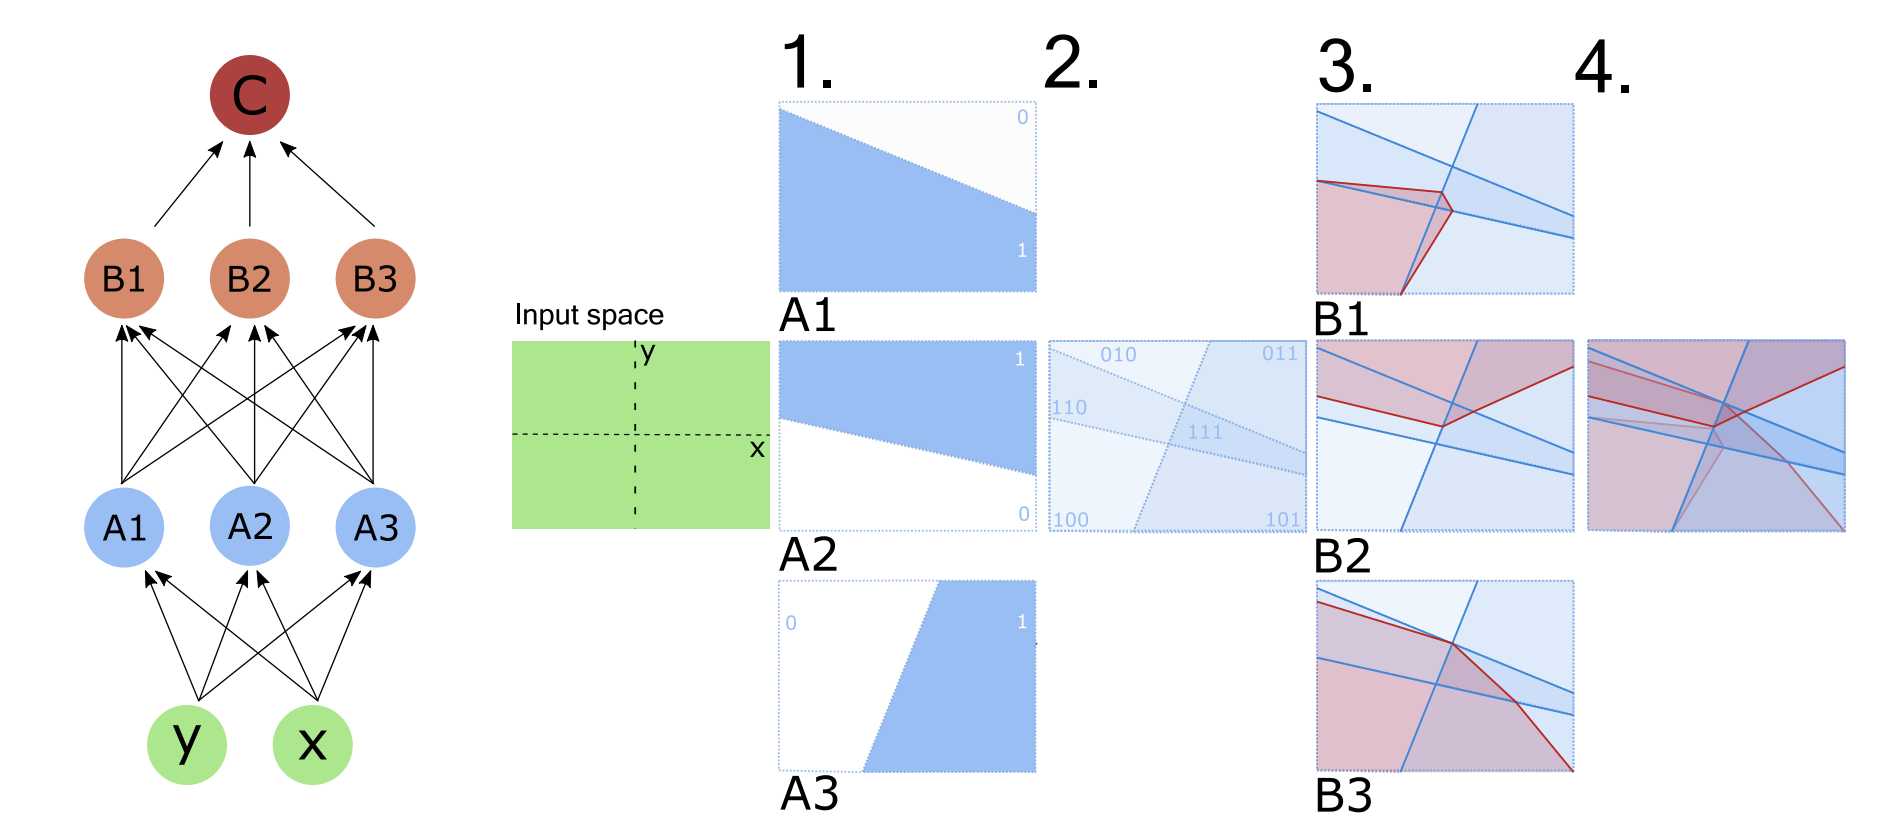
\includegraphics[scale=0.32]{images/figure2.png}
        \caption{Visualising how binary activation codes of ReLU units correspond to linear regions. 1: Each ReLU node Ai splits the input into an active and inactive region We label the active region 1 and inactive 0.
        4: Each linear region at a given node can be uniquely defined by the activation pattern of all the ReLU nodes that preceded it}
        \label{fig:enter-label}
    \end{figure}
\end{frame}


\begin{frame}{Scoring Networks at Initialisation}
    \begin{block}{}
        The objective is to score network architectures at initialisation to predict their final trained accuracy without the costly training process.
        \begin{itemize}
            \item A neural network with ReLU units assigns binary codes to inputs, indicating active and inactive states.
            \item A mini-batch \( X = \{x_i\}_{i=1}^N \) generates binary codes \( \{c_i\} \) per input \( x_i \), defining the linear regions.
            \item The Hamming distance between these codes measures input dissimilarity, used to construct a kernel matrix \( K_H \).
        \end{itemize}
        \begin{equation}
            K_H = \begin{pmatrix}
            N_A - d_H(c_1, c_1) & \cdots & N_A - d_H(c_1, c_N) \\
            \vdots & \ddots & \vdots \\
            N_A - d_H(c_N, c_1) & \cdots & N_A - d_H(c_N, c_N)
            \end{pmatrix}
        \end{equation}
        \begin{itemize}
            \item Networks are scored by \( s = \log |K_H| \), relating to the likelihood of higher final accuracy. This score has shown positive correlation with validation accuracy across multiple datasets and search spaces.
        \end{itemize}
    \end{block}
\end{frame}

\begin{frame}{Scoring Networks at Initialisation}
    \begin{block}{}
        \begin{figure}{}
            \centering
            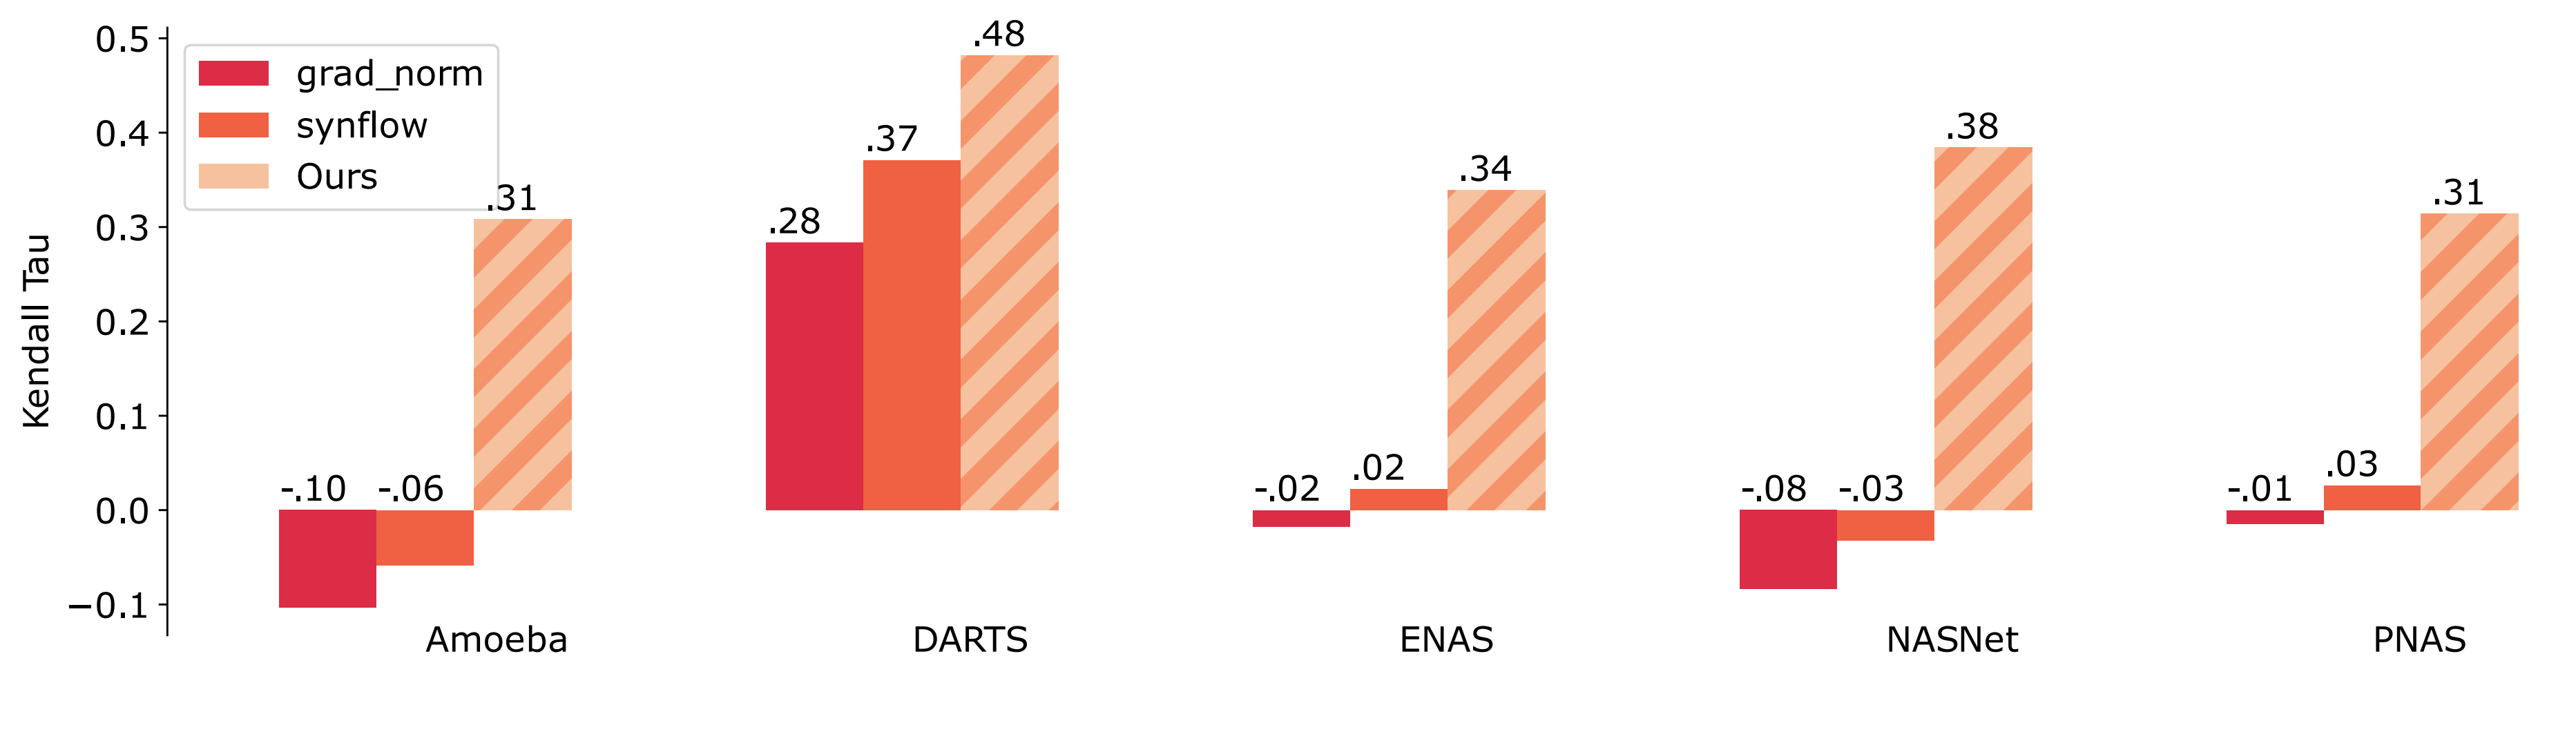
\includegraphics[scale=0.17]{images/figure4.png}
            \caption{Kendall’s Tau correlation across each of the NDS CIFAR-10 search spaces vs alternative measures: grad norm (Euclidean-norm of the gradients over random mini-batch data) and synflow (Tanaka et al. (2020))}
            \label{fig:enter-label}
        \end{figure}
    \end{block}
\end{frame}

\begin{frame}{Scoring Networks at Initialisation}
    \begin{block}{}
        \begin{figure}{}
            \centering
            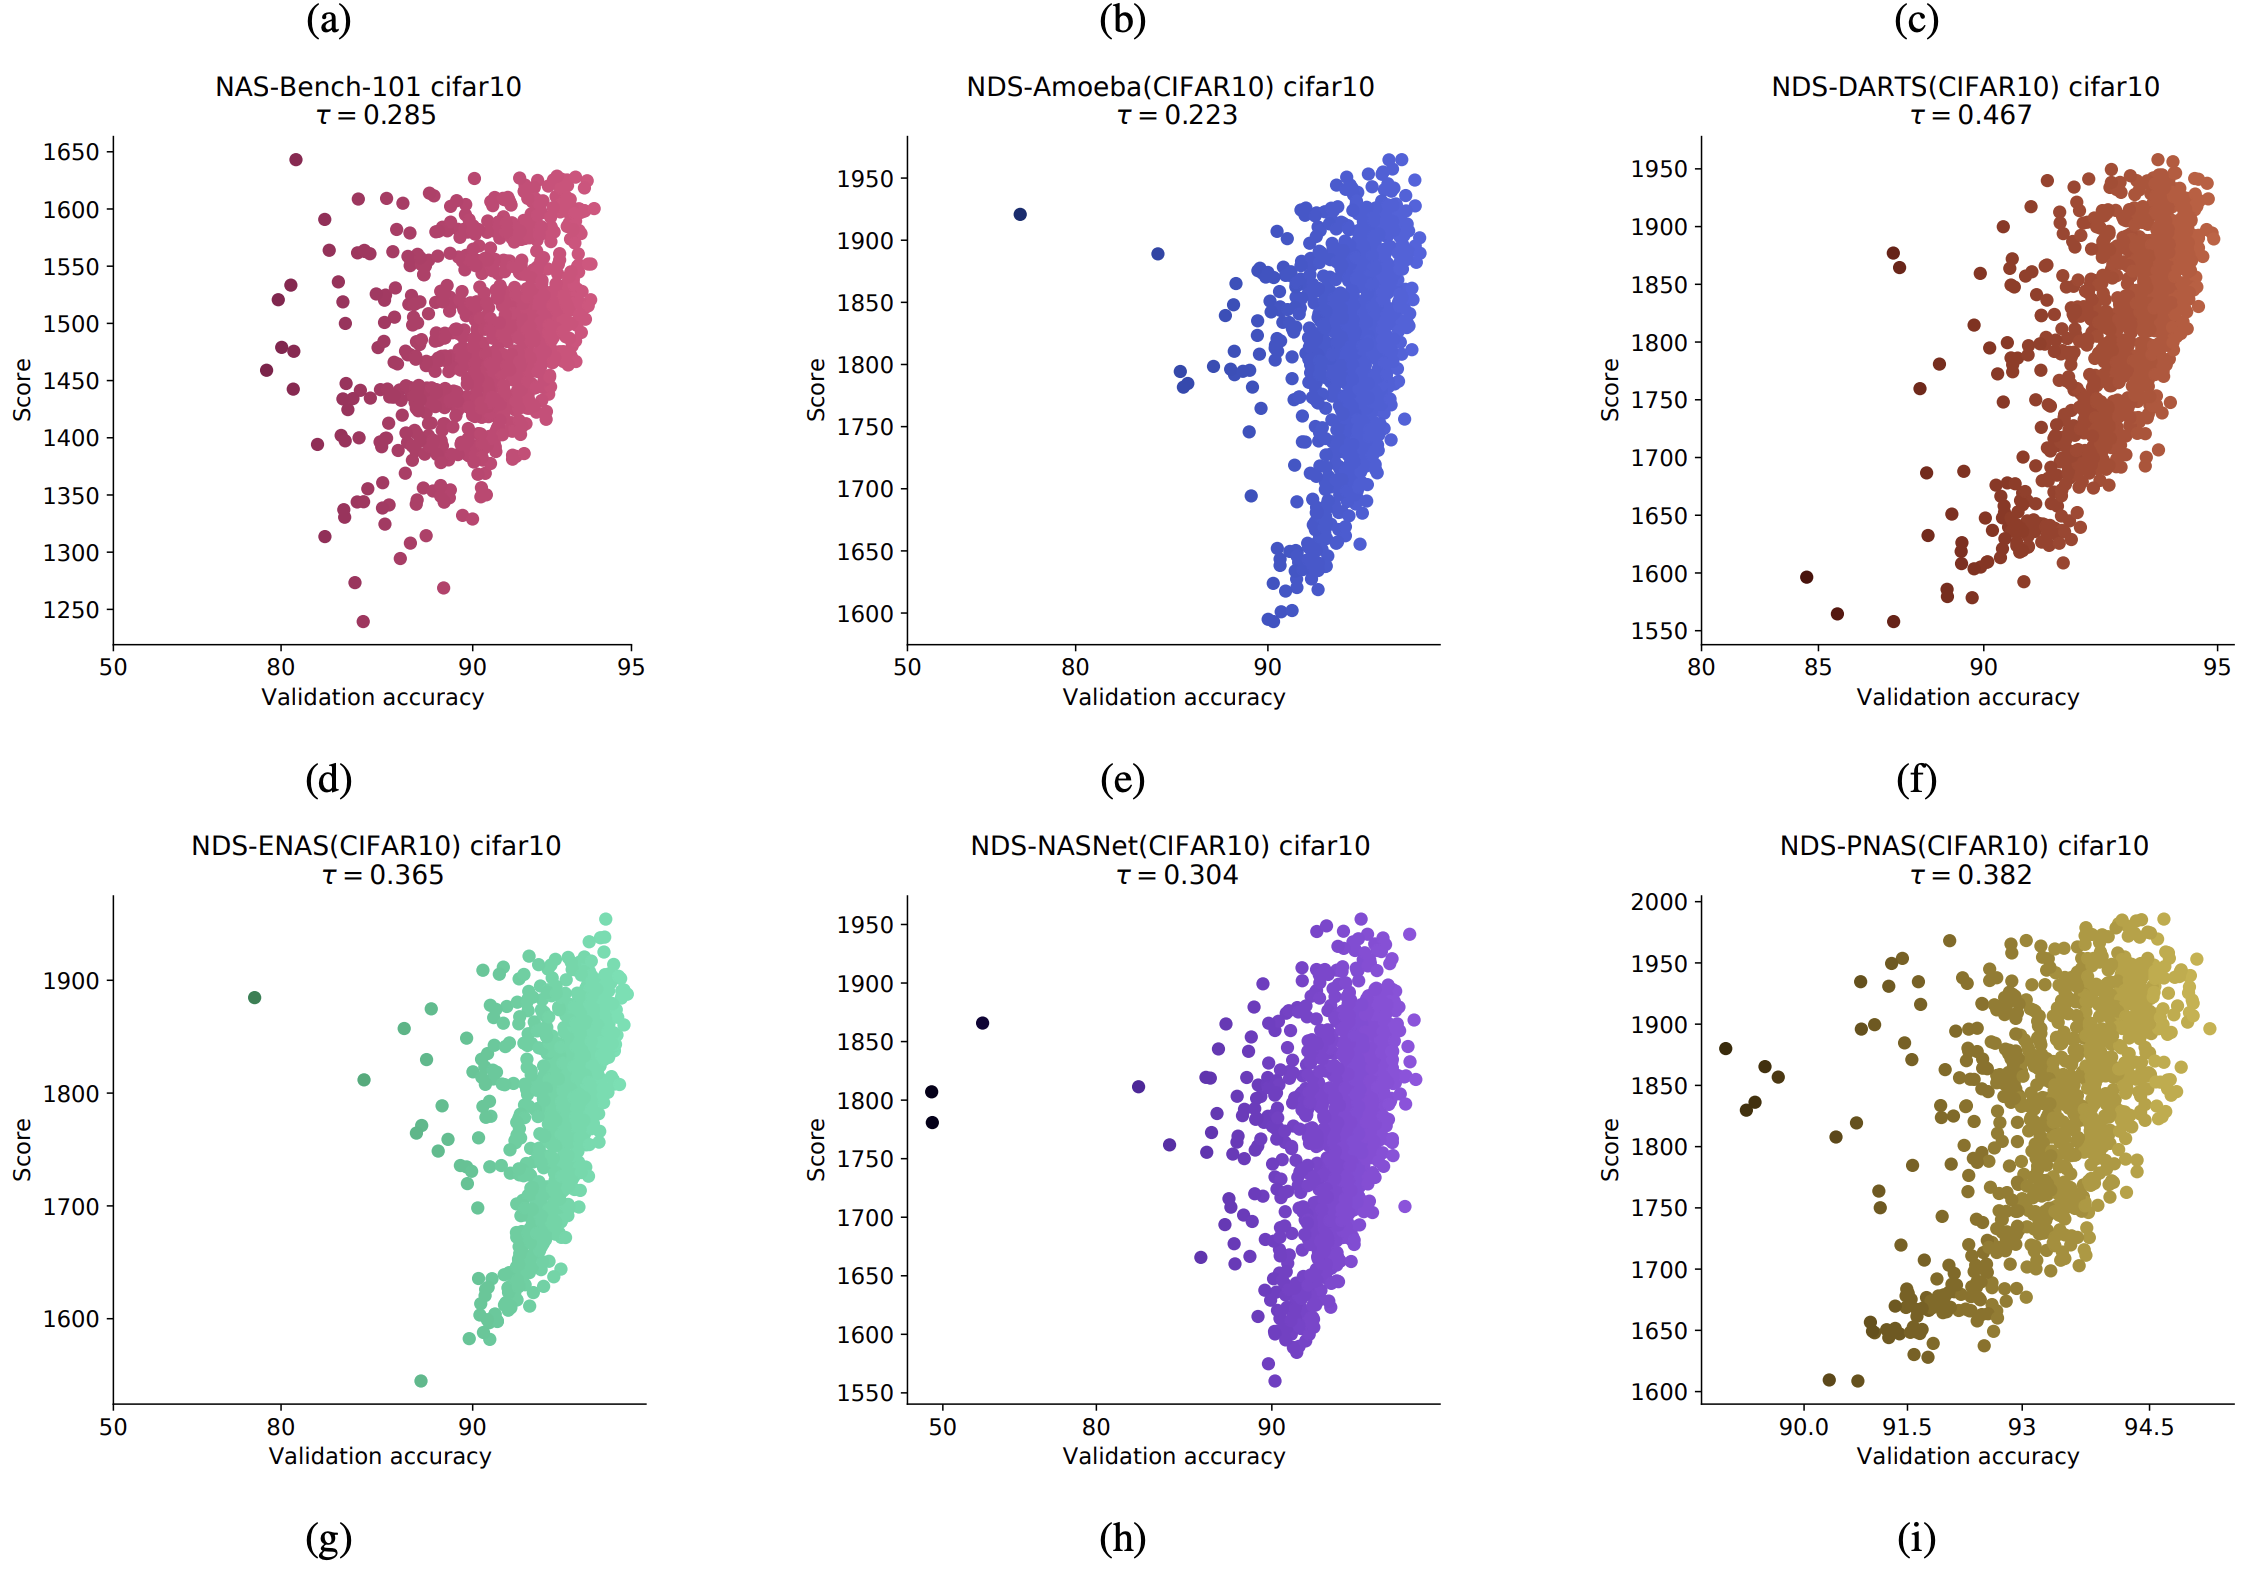
\includegraphics[scale=0.23]{images/figure3.png}
            \caption{Plots of our score for randomly sampled untrained architectures against validation accuracy when trained}
            \label{fig:enter-label}
        \end{figure}
    \end{block}
\end{frame}

\begin{frame}{Scoring Networks at Initialisation}
    \begin{block}{}
        \begin{figure}{}
            \centering
            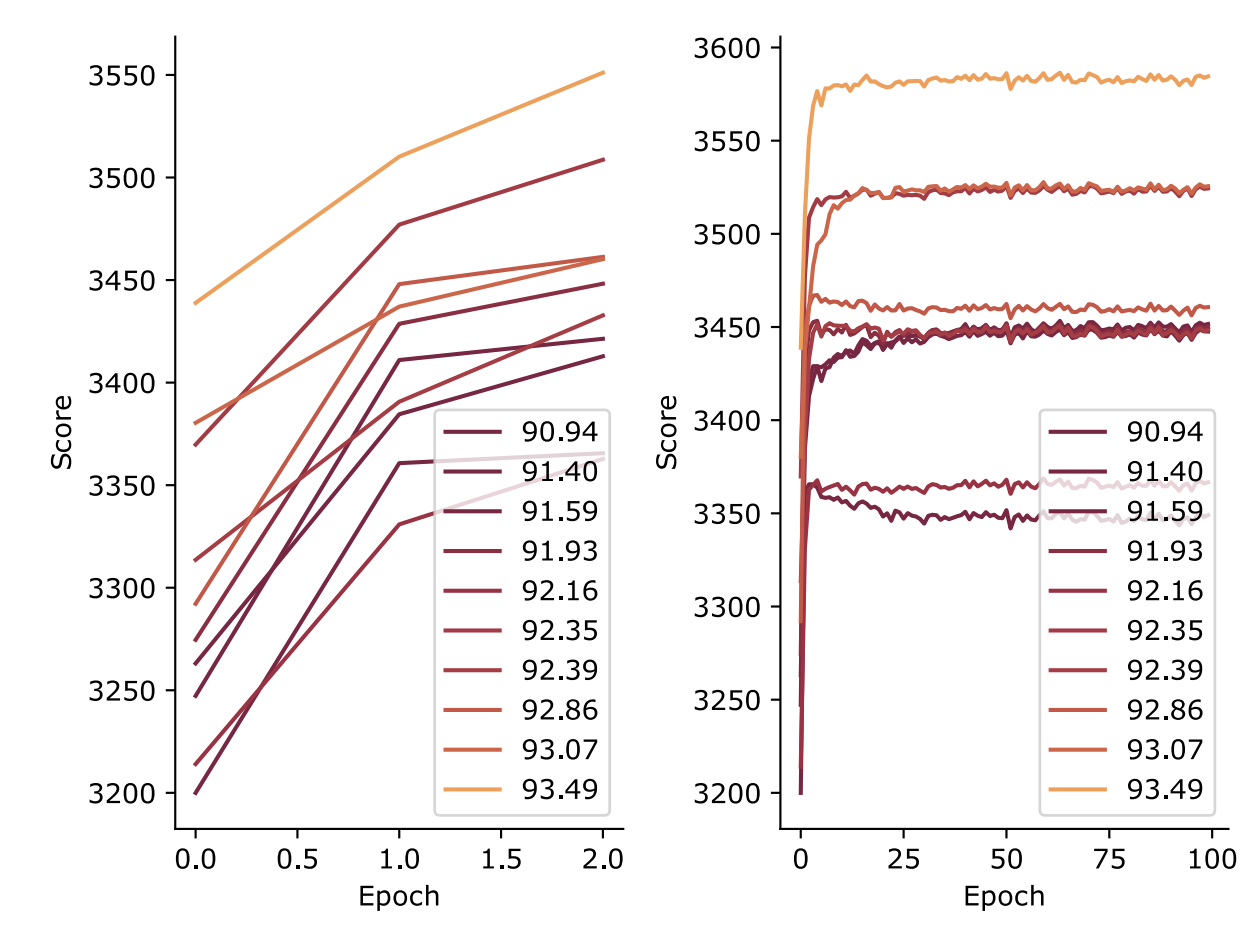
\includegraphics[scale=0.27]{images/figure6.png}
            \caption{Plots of our score during training for 10
networks from NAS-Bench-201 using the CIFAR-10 dataset. For all 10 networks the score increases sharply in the first few epochs and then flattens. The ranking of the scores between networks remains relatively stable throughout
training}
            \label{fig:enter-label}
        \end{figure}
    \end{block}
\end{frame}

\begin{frame}{NASWOT Algorithm}
    \begin{algorithm}[H]
        \caption{NASWOT}
        \begin{algorithmic}
            \State $generator \gets \text{RandomGenerator()}$ 
            
            \State $best\_net, best\_score \gets \text{None}, 0$ 
            
            \For{$i \gets 1 \text{ to } N$}
                \State $net \gets generator.generate()$
                \State $score \gets net.score()$
                \If{$score > best\_score$}
                    \State $best\_net, best\_score \gets net, score$
                \EndIf
            \EndFor
            \State $chosen\_net \gets best\_net$
        \end{algorithmic}
    \end{algorithm}
\end{frame}


\begin{frame}[shrink]
\frametitle{Algorithm 2: Assisted Regularised EA — AREA}
    \begin{algorithm}[H]
        \caption{Assisted Regularised EA — AREA}
        \begin{algorithmic}[1] % The [1] here is to show line numbers
            \State $population \gets []$
            \State $generator \gets \text{RandomGenerator()}$
            \For{$i \gets 1 \text{ to } M$}
                \State $net \gets generator.generate()$
                \State $scored\_net \gets net.score()$
                \State $population.append(scored\_net)$
            \EndFor
            \State Keep the top $N$ scored networks in the population
            \State $history \gets []$
            \For{$net \text{ in } population$}
                \State $trained\_net \gets net.train()$
                \State $history.append(trained\_net)$
            \EndFor
            \While{time limit not exceeded}
                \State Sample sub-population, $S$, without replacement from population
                \State Select network in $S$ with highest accuracy as parent
                \State Mutate parent network to produce child
                \State Train child network
                \State Remove oldest network from population
                \State $population.append(child\ network)$
                \State $history.append(child\ network)$
            \EndWhile
            \State $chosen\_net \gets$ Network in history with highest accuracy
        \end{algorithmic}
    \end{algorithm}
\end{frame}

\section{Results}
\begin{frame}{Results}
    \begin{figure}{}
        \centering
        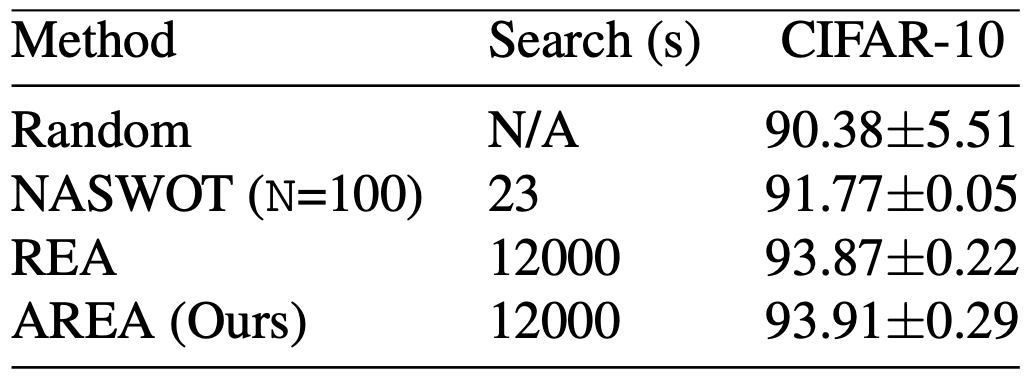
\includegraphics[scale=0.45]{images/table_small.png}
        \caption{Table 1. Mean ± std. accuracy from NAS-Bench-101. NASWOT is our training-free algorithm (across 500 runs). REA uses evolutionary search to select an architecture (50 runs), Random selects one architecture (500 runs). AREA (assisted-REA) uses our score to select the starting population for REA (50 runs). Search times for REA and AREA were calculated using the NASBench-101 API}
        \label{fig:enter-label}
    \end{figure}
\end{frame}

\begin{frame}{Results}
    \begin{block}{}
        \begin{figure}{}
            \centering
            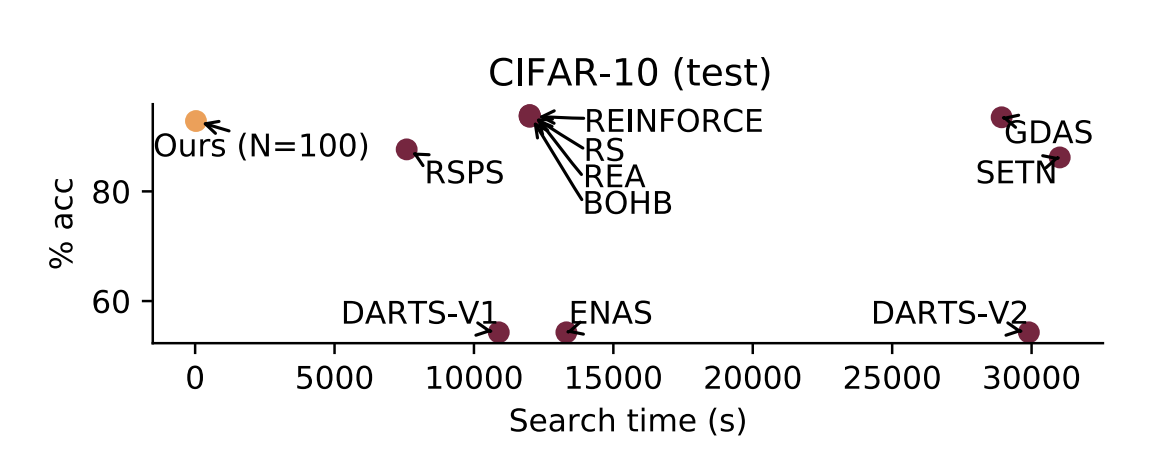
\includegraphics[scale=0.48]{images/figure7.png}
            \caption{Plot showing the search time (as measured using a 1080Ti) against final accuracy of the proposed NAS-Bench-201 network for a number of search strategies}
            \label{fig:enter-label}
        \end{figure}
    \end{block}
\end{frame}

\begin{frame}{Literature}
    \begin{enumerate}
        \item \textbf{Main article} \href{https://arxiv.org/pdf/2006.04647v3.pdf} 
        {Neural Architecture Search without Training}.
    \end{enumerate}
\end{frame}

\end{document}